\paper{2016}

\question
\begin{parts}
    \part[5]
    Give a formal definition of a determinsitic finite-state automaton (DFA).
    \begin{solution}
        A \textbf{DFA} is a $5$-tuple $(Q, \Sigma, \delta, q_0, F)$
        where
        \begin{enumerate}
            \item $Q$ is a finite set of states;
            \item $\Sigma$ is a finite alphabet;
            \item $\delta: Q \times \Sigma \to Q$
                is a transition function;
            \item $q_0 \in Q$ is the initial state; and
            \item $F \subset Q$ is a set of accept states.
        \end{enumerate}
    \end{solution}

    \part[8]
    Consider the non-deterministic finite-state automaton (NFA)
    whose transition function is given in the table below
    \begin{center}
        \begin{tabular}{cccc}
            \toprule
              & $A$ & $B$ & $C$ \\
            \midrule
            0 & $A,B$ &       & $C$ \\
            1 & $C$   & $B,C$ & $A$ \\
            \bottomrule
        \end{tabular}
    \end{center}
    and where $A$ is the start state, 
    and $C$ is the only accepting state.
    Convert this NFA to a regular expression.
    Show your working.
    \begin{solution}
        \begin{center}
            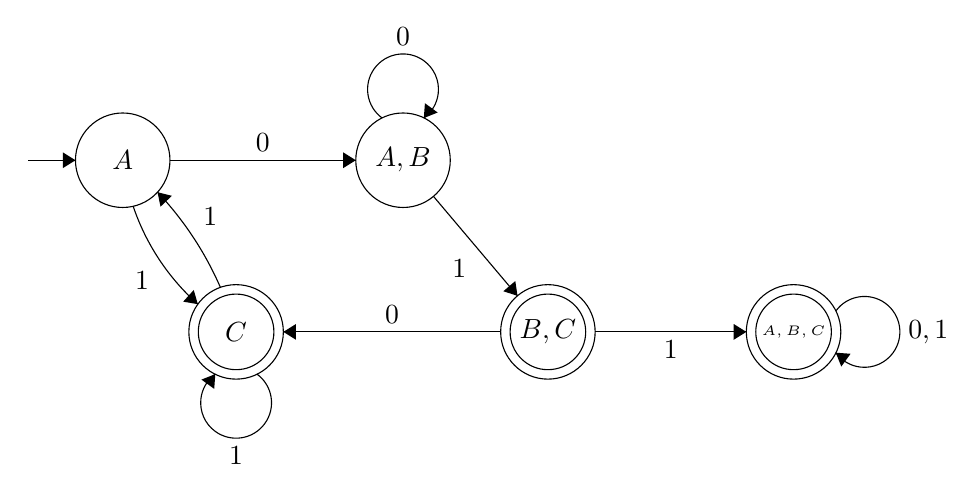
\begin{tikzpicture}[scale=0.2]
                \tikzstyle{every node}+=[inner sep=0pt]
                \draw [black] (12.2,-23.3) circle (3);
                \draw (12.2,-23.3) node {$A$};
                \draw [black] (30,-23.3) circle (3);
                \draw (30,-23.3) node {$A,B$};
                \draw [black] (19.4,-34.2) circle (3);
                \draw (19.4,-34.2) node {$C$};
                \draw [black] (19.4,-34.2) circle (2.4);
                \draw [black] (39.2,-34.2) circle (3);
                \draw (39.2,-34.2) node {$B,C$};
                \draw [black] (39.2,-34.2) circle (2.4);
                \draw [black] (54.8,-34.2) circle (3);
                \draw (54.8,-34.2) node {\tiny$A,B,C$};
                \draw [black] (54.8,-34.2) circle (2.4);
                \draw [black] (6.2,-23.3) -- (9.2,-23.3);
                \fill [black] (9.2,-23.3) -- (8.4,-22.8) -- (8.4,-23.8);
                \draw [black] (15.2,-23.3) -- (27,-23.3);
                \fill [black] (27,-23.3) -- (26.2,-22.8) -- (26.2,-23.8);
                \draw (21.1,-22.8) node [above] {$0$};
                \draw [black] (16.974,-32.444) arc (-131.77823:-161.32822:14.624);
                \fill [black] (16.97,-32.44) -- (16.71,-31.54) -- (16.04,-32.28);
                \draw (13.9,-30.93) node [left] {$1$};
                \draw [black] (14.409,-25.326) arc (43.3811:23.51245:21.004);
                \fill [black] (14.41,-25.33) -- (14.6,-26.25) -- (15.32,-25.56);
                \draw (17.28,-26.85) node [right] {$1$};
                \draw [black] (28.677,-20.62) arc (234:-54:2.25);
                \draw (30,-16.05) node [above] {$0$};
                \fill [black] (31.32,-20.62) -- (32.2,-20.27) -- (31.39,-19.68);
                \draw [black] (31.93,-25.59) -- (37.27,-31.91);
                \fill [black] (37.27,-31.91) -- (37.13,-30.97) -- (36.37,-31.62);
                \draw (34.05,-30.19) node [left] {$1$};
                \draw [black] (42.2,-34.2) -- (51.8,-34.2);
                \fill [black] (51.8,-34.2) -- (51,-33.7) -- (51,-34.7);
                \draw (47,-34.7) node [below] {$1$};
                \draw [black] (57.48,-32.877) arc (144:-144:2.25);
                \draw (62.05,-34.2) node [right] {$0,1$};
                \fill [black] (57.48,-35.52) -- (57.83,-36.4) -- (58.42,-35.59);
                \draw [black] (36.2,-34.2) -- (22.4,-34.2);
                \fill [black] (22.4,-34.2) -- (23.2,-34.7) -- (23.2,-33.7);
                \draw (29.3,-33.7) node [above] {$0$};
                \draw [black] (20.723,-36.88) arc (54:-234:2.25);
                \draw (19.4,-41.45) node [below] {$1$};
                \fill [black] (18.08,-36.88) -- (17.2,-37.23) -- (18.01,-37.82);
            \end{tikzpicture}
        \end{center}
    \end{solution}

    \part[5]
    Prove that the language
    \[
        \{
            a^{2^n} : n \in \N
        \}
    \]
    is not context-free.
    \begin{solution}
        Assume the language above, $L$, is context-free.
        Then $L$ is regular.
        Consider $w = a^{2^p} \in L$ where $p$ is the pumping length
        of $L$.
        Now, by the pumping lemma we have
        $w = a^la^ma^{2^p-l-m}$
        where $l,m \in \Z_{\geq 0}$ and
        \begin{enumerate}
            \item $m \geq 1$;
            \item $l + m \leq p$; and
            \item $a^l(a^m)^ia^{2^p-l-m} \in L$ for all $i \geq 0$.
        \end{enumerate}
        By (ii) we get $m \leq p$.
        (iii) is satisfied if and only if $2^p + (i-1)m = 2^n$ for some $n \in \N$.
        Now, for $i = 2$, we have
        \[
            2^p + m \leq 2^p + p \leq 2^p + 2^p = 2^{p+1}.
        \]
        In fact, we have $2^p + m < 2^{p+1}$ as
        $m \leq p$ implies that $m \neq 2^p$.
        Indeed we also have $2^p < 2^p + m$;
        so $2^p + m$ lies in between two powers of $2$;
        hence,
        $a^l(a^m)^ia^{2^p-l-m} \not \in L$
        for $i = 2$, a contradiction.
        Therefore, $L$ is not context-free.
    \end{solution}

    \part[7]
    Is it semi-decidable to test whether a Turing-decidable 
    language is empty?
    Justify your answer.
    \begin{solution}
        By Rice's theorem, it certainly is not deciable.
        The complement, testing whether a Turing-deciable 
        language is non-empty is clearly semi-deciable.
        If both a language and its complement are semi-deciable, 
        then it must be deciable; therefore,
        the set of Turing machine with an empty language is not semi-deciable.
    \end{solution}
\end{parts}

\question
\begin{parts}
    \part[6]
    Give a formal definition of an NFA.
    \begin{solution}
        A \textbf{NFA} is a $5$-tuple $(Q, \Sigma, \delta, q_0, F)$
        where
        \begin{enumerate}
            \item $Q$ is a finite set of states;
            \item $\Sigma$ is a finite alphabet;
            \item $\delta: Q \times \Sigma \to \mathcal P(Q)$
                is a transition function;
            \item $q_0 \in Q$ is an initial state; and
            \item $F \subset Q$ is a set of accept states.
        \end{enumerate}
    \end{solution}

    \part[8]
    Minimise the DFA whose transition function 
    is given in the table below
    \begin{center}
        \begin{tabular}{cccccccccc}
            \toprule
              & $A$ & $B$ & $C$ & $D$ & $E$ & $F$ & $G$ & $H$ & $I$ \\
            \midrule
            0 & $G$ & $C$ & $D$ & $I$ & $A$ & $I$ & $I$ & $E$ & $C$ \\
            1 & $B$ & $E$ & $B$ & $A$ & $I$ & $G$ & $C$ & $G$ & $B$ \\
            \bottomrule
        \end{tabular}
    \end{center}
    and where $A$ is the start state, and $D, G$ are the accepting states.
    Show your working.
    \begin{solution}
        \begin{center}
            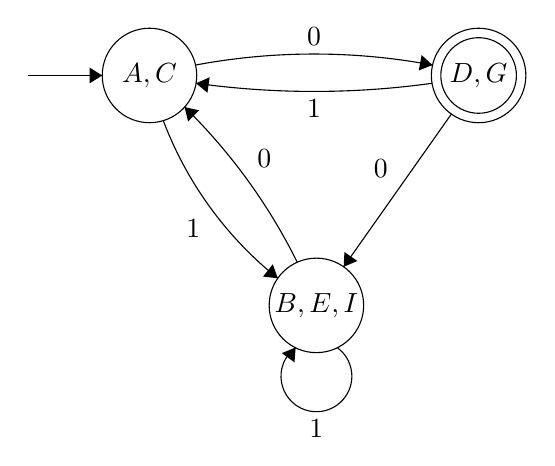
\begin{tikzpicture}[scale=0.2]
                \tikzstyle{every node}+=[inner sep=0pt]
                \draw [black] (12.7,-24.4) circle (3);
                \draw (12.7,-24.4) node {$A,C$};
                \draw [black] (33.6,-24.4) circle (3);
                \draw (33.6,-24.4) node {$D,G$};
                \draw [black] (33.6,-24.4) circle (2.4);
                \draw [black] (23.3,-39) circle (3);
                \draw (23.3,-39) node {$B,E,I$};
                \draw [black] (5,-24.4) -- (9.7,-24.4);
                \fill [black] (9.7,-24.4) -- (8.9,-23.9) -- (8.9,-24.9);
                \draw [black] (15.625,-23.738) arc (100.63663:79.36337:40.766);
                \fill [black] (30.67,-23.74) -- (29.98,-23.1) -- (29.8,-24.08);
                \draw (23.15,-22.54) node [above] {$0$};
                \draw [black] (30.642,-24.895) arc (-82.07486:-97.92514:54.334);
                \fill [black] (15.66,-24.9) -- (16.38,-25.5) -- (16.52,-24.51);
                \draw (23.15,-25.91) node [below] {$1$};
                \draw [black] (20.846,-37.278) arc (-128.72826:-159.31038:23.455);
                \fill [black] (20.85,-37.28) -- (20.53,-36.39) -- (19.91,-37.17);
                \draw (15.95,-34.14) node [left] {$1$};
                \draw [black] (14.929,-26.407) arc (45.62622:26.33514:36.333);
                \fill [black] (14.93,-26.41) -- (15.15,-27.32) -- (15.85,-26.61);
                \draw (19.51,-29.65) node [right] {$0$};
                \draw [black] (31.87,-26.85) -- (25.03,-36.55);
                \fill [black] (25.03,-36.55) -- (25.9,-36.18) -- (25.08,-35.61);
                \draw (27.86,-30.33) node [left] {$0$};
                \draw [black] (24.623,-41.68) arc (54:-234:2.25);
                \draw (23.3,-46.25) node [below] {$1$};
                \fill [black] (21.98,-41.68) -- (21.1,-42.03) -- (21.91,-42.62);
            \end{tikzpicture}
        \end{center}
    \end{solution}

    \part[7]
    Explain how a correctly formed arithmetic expression over the variables
    $a$, $b$, and $c$ that contains additions,
    multiplications, square brackets, and curly brackets
    can be recognised by a PDA.
    \begin{solution}
        % todo
    \end{solution}

    \part[4]
    Give an algorithm that decides whether $L(M_1) = \overline{L(M_2)}$
    for any two DFAs $M_1$ and $M_2$.
    (Here $L(M_i)$ denotes the language recognised by $M_i$
    and $\overline A$ denotes the complement of $A$.)
    \begin{solution}
        % todo
    \end{solution}
\end{parts}

\question
\begin{parts}
    \part[7]
    Give a formal definition of a push-down automaton (PDA).
    \begin{solution}
        % todo
    \end{solution}

    \part[7]
    Consider the NFA whose tranisition function is given in the 
    table below,
    and where $A$ is the start state and $D$ is the only accept state.
    \begin{center}
        \begin{tabular}{ccccc}
            \toprule
                          & $A$   & $B$ & $C$ & $D$ \\
            \midrule
            $a$           & $A,C$ & $D$ &     &     \\
            $b$           & $A$   &     & $B$ &     \\
            $\varepsilon$ &       &     & $B$ &     \\
            \bottomrule
        \end{tabular}
    \end{center}
    Transform this NFA into a DFA.
    Show your working.
    \begin{solution}
        \begin{center}
            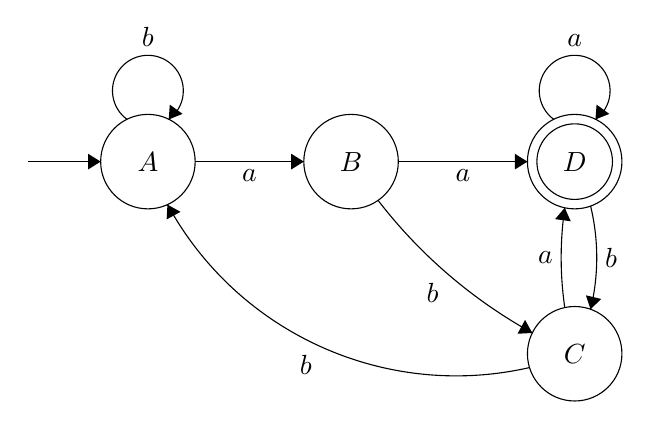
\begin{tikzpicture}[scale=0.2]
                \tikzstyle{every node}+=[inner sep=0pt]
                \draw [black] (15.3,-21.6) circle (3);
                \draw (15.3,-21.6) node {$A$};
                \draw [black] (28.2,-21.6) circle (3);
                \draw (28.2,-21.6) node {$B$};
                \draw [black] (42.4,-21.6) circle (3);
                \draw (42.4,-21.6) node {$D$};
                \draw [black] (42.4,-21.6) circle (2.4);
                \draw [black] (42.4,-33.8) circle (3);
                \draw (42.4,-33.8) node {$C$};
                \draw [black] (7.7,-21.6) -- (12.3,-21.6);
                \fill [black] (12.3,-21.6) -- (11.5,-21.1) -- (11.5,-22.1);
                \draw [black] (18.3,-21.6) -- (25.2,-21.6);
                \fill [black] (25.2,-21.6) -- (24.4,-21.1) -- (24.4,-22.1);
                \draw (21.75,-22.1) node [below] {$a$};
                \draw [black] (13.977,-18.92) arc (234:-54:2.25);
                \draw (15.3,-14.35) node [above] {$b$};
                \fill [black] (16.62,-18.92) -- (17.5,-18.57) -- (16.69,-17.98);
                \draw [black] (31.2,-21.6) -- (39.4,-21.6);
                \fill [black] (39.4,-21.6) -- (38.6,-21.1) -- (38.6,-22.1);
                \draw (35.3,-22.1) node [below] {$a$};
                \draw [black] (41.077,-18.92) arc (234:-54:2.25);
                \draw (42.4,-14.35) node [above] {$a$};
                \fill [black] (43.72,-18.92) -- (44.6,-18.57) -- (43.79,-17.98);
                \draw [black] (43.41,-24.419) arc (13.57166:-13.57166:13.983);
                \fill [black] (43.41,-30.98) -- (44.08,-30.32) -- (43.11,-30.09);
                \draw (44.3,-27.7) node [right] {$b$};
                \draw [black] (41.77,-30.869) arc (-171.76199:-188.23801:22.118);
                \fill [black] (41.77,-24.53) -- (41.16,-25.25) -- (42.15,-25.39);
                \draw (41.04,-27.7) node [left] {$a$};
                \draw [black] (39.71,-32.475) arc (-118.9245:-142.41088:31.724);
                \fill [black] (39.71,-32.48) -- (39.25,-31.65) -- (38.77,-32.53);
                \draw (33.37,-29.26) node [below] {$b$};
                \draw [black] (39.534,-34.677) arc (-77.10384:-151.36923:20.883);
                \fill [black] (16.54,-24.33) -- (16.49,-25.27) -- (17.37,-24.79);
                \draw (25.32,-33.87) node [below] {$b$};
            \end{tikzpicture}   
        \end{center}
        Here: $A = \{A\}$, $B = \{A,B,C\}$, $C=\{A,B\}$, and $D=\{A,B,C,D\}$.
    \end{solution}

    \part[7]
    For every two strings $u$ and $v$, we say that $u$
    is a subsequence of $v$ if $u$ can be produced by removing zero
    or more characters from $v$.
    Show that the language
    \[
        \{
            u\#v : u,v \in \{a,b\}^\star, \text{$u$ is a subsequence of $v$}
        \}
    \]
    is context-sensitive.
    \begin{solution}
        \emph{Pretty sure this isn't covered.}
    \end{solution}

    \part[4]
    Give an algorithm that decides if a given DFA accepts at least one
    word of even length.
    \begin{solution}
        Given an alphabet $\Sigma$,
        for all $w \in \Sigma^\star$ such that $\abs w$ is even,
        run the DFA on the input. If it accepts,
        otherwise move onto the next $w$.
    \end{solution}
\end{parts}

\question
\begin{parts}
    \part[6]
    Give a formal definition of a context-free grammar (CFG).
    \begin{solution}
        \emph{Context not covered, maybe.}
    \end{solution}

    \part[7]
    Prove that the language
    \[
        \{
            u1v: u,v \in \{0,1\}^\star, \abs u = 2 \abs v
        \}
    \]
    is not regular.
    \begin{solution}
        Assume the language above, $L$, is regular.
        Let $p$ be the pumping length of $L$.
        Consider $w = 0^p10^{2p} \in L$.
        By the pumping lemma,
        $w = xyz$
        for $x,y,z \in L$ where
        \begin{enumerate}
            \item $\abs y \geq 1$;
            \item $\abs{xy} \leq p$; and
            \item $xy^iz \in L$ for all $i \geq 0$.
        \end{enumerate}
        Therefore, $x = 0^l$, $y = 0^m$, and $z = 0^{p-l-m}10^{2p}$
        for some $l \geq 0$, $m \geq 1$.
        We have
        \[
            xy^0z = xz = 0^{p-m}10^{2p}
        \]
        but as $m \neq 0$, $2(p-m) \neq 2p$ so $xy^0z \not\in L$,
        a contradiction to (iii);
        therefore, $L$ is not regular.
    \end{solution}

    \part[7]
    Design a DFA that recognises precisely the words that contain the
    string
    \emph{``baabbab''}
    as a subword.
    \begin{solution}
        \begin{center}
            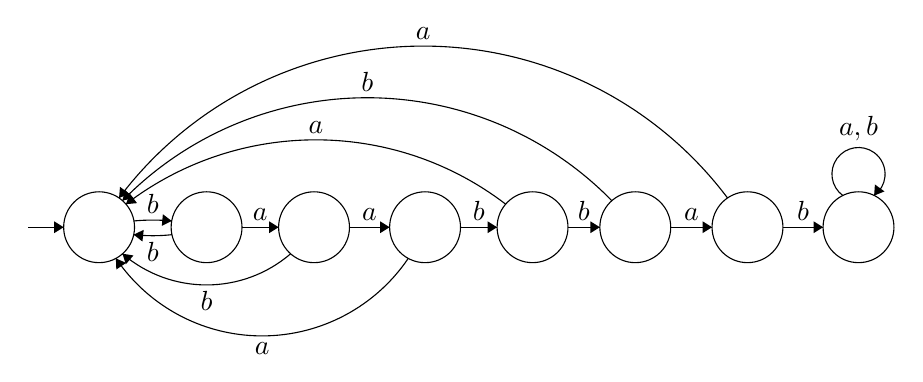
\begin{tikzpicture}[scale=0.15]
                \tikzstyle{every node}+=[inner sep=0pt]
                \draw [black] (8.1,-26.4) circle (3);
                \draw [black] (17.2,-26.4) circle (3);
                \draw [black] (26.3,-26.4) circle (3);
                \draw [black] (35.7,-26.4) circle (3);
                \draw [black] (44.8,-26.4) circle (3);
                \draw [black] (53.5,-26.4) circle (3);
                \draw [black] (63,-26.4) circle (3);
                \draw [black] (72.4,-26.4) circle (3);
                \draw [black] (2.1,-26.4) -- (5.1,-26.4);
                \fill [black] (5.1,-26.4) -- (4.3,-25.9) -- (4.3,-26.9);
                \draw [black] (71.077,-23.72) arc (234:-54:2.25);
                \draw (72.4,-19.15) node [above] {$a,b$};
                \fill [black] (73.72,-23.72) -- (74.6,-23.37) -- (73.79,-22.78);
                \draw [black] (11.049,-25.868) arc (95.28368:84.71632:17.389);
                \fill [black] (14.25,-25.87) -- (13.5,-25.3) -- (13.41,-26.29);
                \draw (12.65,-25.29) node [above] {$b$};
                \draw [black] (20.2,-26.4) -- (23.3,-26.4);
                \fill [black] (23.3,-26.4) -- (22.5,-25.9) -- (22.5,-26.9);
                \draw (21.75,-25.9) node [above] {$a$};
                \draw [black] (29.3,-26.4) -- (32.7,-26.4);
                \fill [black] (32.7,-26.4) -- (31.9,-25.9) -- (31.9,-26.9);
                \draw (31,-25.9) node [above] {$a$};
                \draw [black] (38.7,-26.4) -- (41.8,-26.4);
                \fill [black] (41.8,-26.4) -- (41,-25.9) -- (41,-26.9);
                \draw (40.25,-25.9) node [above] {$b$};
                \draw [black] (47.8,-26.4) -- (50.5,-26.4);
                \fill [black] (50.5,-26.4) -- (49.7,-25.9) -- (49.7,-26.9);
                \draw (49.15,-25.9) node [above] {$b$};
                \draw [black] (56.5,-26.4) -- (60,-26.4);
                \fill [black] (60,-26.4) -- (59.2,-25.9) -- (59.2,-26.9);
                \draw (58.25,-25.9) node [above] {$a$};
                \draw [black] (66,-26.4) -- (69.4,-26.4);
                \fill [black] (69.4,-26.4) -- (68.6,-25.9) -- (68.6,-26.9);
                \draw (67.7,-25.9) node [above] {$b$};
                \draw [black] (14.272,-27.03) arc (-83.6883:-96.3117:14.755);
                \fill [black] (11.03,-27.03) -- (11.77,-27.61) -- (11.88,-26.62);
                \draw (12.65,-27.62) node [below] {$b$};
                \draw [black] (24.322,-28.643) arc (-49.27342:-130.72658:10.916);
                \fill [black] (10.08,-28.64) -- (10.36,-29.54) -- (11.01,-28.79);
                \draw (17.2,-31.79) node [below] {$b$};
                \draw [black] (34.278,-29.036) arc (-34.10604:-145.89396:14.949);
                \fill [black] (9.52,-29.04) -- (9.56,-29.98) -- (10.39,-29.42);
                \draw (21.9,-36.1) node [below] {$a$};
                \draw [black] (10.374,-24.446) arc (127.42748:52.57252:26.451);
                \fill [black] (10.37,-24.45) -- (11.31,-24.36) -- (10.71,-23.56);
                \draw (26.45,-18.5) node [above] {$a$};
                \draw [black] (10.083,-24.151) arc (135.62938:44.37062:28.981);
                \fill [black] (10.08,-24.15) -- (11,-23.93) -- (10.29,-23.23);
                \draw (30.8,-14.94) node [above] {$b$};
                \draw [black] (9.789,-23.922) arc (143.05445:36.94555:32.233);
                \fill [black] (9.79,-23.92) -- (10.67,-23.58) -- (9.87,-22.98);
                \draw (35.55,-10.56) node [above] {$a$};
            \end{tikzpicture}
        \end{center}
    \end{solution}

    \part[5]
    Consider the following problem.
    \begin{center}
        \itshape
        ``Given a Turing machine, does it terminate on some input?''
    \end{center}
    Show that this problem is semi-decidable.
    \begin{solution}
        Let $M$ be a Turing machine and $w$ be some input to that Turing machine.
        Then we construct a Turing machine $U$ 
        that simulates $M$ on $w$, if it halts on the input accept.
        This Turing machine recognises the language
        \[
            \{(M,w): \text{$M$ halts on $w$}\}.
        \]
        and so the problem is semi-decidable.
    \end{solution}
\end{parts}
